\documentclass{article}

\usepackage[paperwidth=190mm,paperheight=330mm, margin={.5in,.6in}]{geometry}
% \usepackage[a4paper, margin={.5in,1in}]{geometry}
\usepackage{amsmath}
\usepackage{mathdots}
\usepackage{graphicx}
\usepackage{tikz}
\usetikzlibrary{arrows,matrix,positioning}
\usetikzlibrary{decorations.markings}
\usetikzlibrary{arrows.meta}
\usetikzlibrary{fit}
\usepackage{amsfonts}
\usepackage{amsthm}
\usepackage{pgfplots}

\theoremstyle{definition}
\newtheorem*{example}{Example}
\theoremstyle{definition}
\newtheorem*{answer}{Answer}

\newtheorem{theorem}{Theorem}[section]
\newtheorem{lemma}[theorem]{Lemma}

\title{Calculus Overview}
\author{Pi Han}

\newcommand{\ltoinf}{\lim_{x \to \infty}}

\newcommand{\sh}{\sinh}
\newcommand{\ch}{\cosh}

\newcommand{\ash}{\operatorname{arcsinh}}
\newcommand{\ach}{\operatorname{arccosh}}
\newcommand{\ath}{\operatorname{arctanh}}

\newcommand{\arccot}{\operatorname{arccot}}

\newcommand{\dd}{\mathrm{d}}

\begin{document}

\maketitle

\section{Limit}

\subsection{Rules for O-notation}

\begin{itemize}
\end{itemize}

Some product is easy to know the coefficient of $x^{\alpha}$ term without collecting
all the terms, for example:
\[
	\prod_{i=1}^n (1 + k_i x^{\alpha}+ O(x^{\alpha+1})) 
	= 1 + \left(\sum_{i=1}^n k_i\right) x^{\alpha} + O(x^{\alpha+1})
\] 
since the $x^{\alpha}$ term only comes from choosing one $k_i x^{\alpha}$ term
from one factor and $1$ from all other factors.

Be careful when tackle composite function, approximate the inner function first may
cause loss of precision, for example, linearly term in the inner function contributes
the outer approximation only linearly: (here we only consider the case when $x \to 0$
both $f$ and $g$ are approximated at $0$)
\[
f(g(x)) = f(g_1 x + g_2 x^2 + O(x^3)) = f_1(g_1 x + g_2 x^2 + O(x^3))
+ O((g_1 x + g_2 x^2 + O(x^3))^2)
\] 
\[
= f_1g_1 x + O(x^2)
\] 
since the outer linear approximation collects all higher order terms into $O(x^2)$,
which comes from the square of $ g_1 x$. 

In another word, if the inner function's lowest order term is $x^{k}$, and 
we approximate the outer function to $O(g^{n})$, then the final
approximation is only precise to $O(x^{kn})$.

That is, when trying to approximate a composite function $f(g(x))$ to m order, we need to
approximate the outer function $f(x)$ to $O(x^{\lceil (m+1)/k \rceil})$, where $k$ is
the lowest order term in the inner function's approximation to m order.
And first approximate the outer function, then substitute the inner function's
approximation.

\begin{example}
	Find the 3nd order approximation of
	\[
	\sin(\sin x)
	\] 
	when approximate the inner function to $O(x^4)$, its lowest order term is $x$,
	so we need to approximate the outer function to $O(x^4)$:
	\[
		\sin(\sin x) = \sin x - \dfrac{(\sin x)^3}{6} + O(x^4)
	\]
	then substitute the inner function's approximation:
	\[
		\sin(\sin x) = x - \dfrac{x^3}{6} - \dfrac{x^3}{6} + O(x^4) = x - \dfrac{x^3}{3} + O(x^4)
	\]
	here we don't need to expand the $(\sin x)^3$ term since only its $x$ term
	contributes to the $x^3$ term in the final approximation, other terms are collected
	into $O(x^4)$.
\end{example}
\begin{example}
	We can also approximate more precisely, using the same method, but need to expand
	the cubic term:
	\[
		\sin(\sin x) = \sin x - \dfrac{\sin^3 x}{6} + \dfrac{\sin^5 x}{120} + O(x^6)
	\] 
	then substitute the inner function's approximation:
	\[
		\begin{aligned}
			\sin(\sin x) &= x - \dfrac{x^3}{6} + \dfrac{x^5}{120}
			- \dfrac{1}{6}\left(x^{3} - \dfrac{3x^5}{6}\right) + \dfrac{1}{120}x^{5} + O(x^6) \\
									 &= x - \dfrac{x^3}{3} + \dfrac{x^5}{10} + O(x^6)
		\end{aligned}
	\]
\end{example}
\begin{example}
For $\ln(1-x^2)$ the error of composite function is not an issue since the inner
function's lowest order term is $x^2$
\[
	\ln(1+x)+\ln(1-x) = \ln(1-x^2) = - x^2 - \dfrac{x^4}{2} - \dfrac{x^6}{3} + O(x^8)
\] 
\end{example}

\subsection{Indeterminate Forms}
\subsubsection{1-$\prod 1$ Forms}
When there are multiple factors tending to $1$, we can use logarithm to convert
the product into sum:
\[
	1-\prod_{i=1}^n u_i \sim -\ln \prod_{i=1}^n u_i = -\sum_{i=1}^n \ln u_i
\]
 \begin{example}
	 Find the limit
	 \[
		 \lim_{x \to 0} \frac{1-\cos x \cos 2x \cos 3x}{x^2}
	 \]
	 we have
	 \[
		 1 - \cos x \cos 2x \cos 3x \sim -\ln(\cos x) - \ln(\cos 2x) - \ln(\cos 3x)
	 \]
	\end{example}
	But be careful when using this method, since it can be hard to determine
the order of the final result.
\subsubsection{$1^\infty$ Indeterminate Form}
When
 \[
	 \lim_{x \to \infty} u = 0 \quad \text{and} \quad
	 \lim_{x \to \infty} v = \infty
\] 
then
\[
	\ltoinf(1+u)^{v} = \exp\left({\ltoinf uv}\right)
\] 
and when
\[
	\ltoinf u = 1 \quad \text{and} \quad \ltoinf v = \infty
\] 
we have
\[
	\ltoinf (u)^{v} = \exp\left({\ltoinf (u-1)v}\right)
\] 
\subsection{Tylor Series Approximation}

\[
	(1+x)^{p} = 1 + px + \dfrac{p(p-1)}{2} x^2 + \dfrac{p(p-1)(p-2)}{3!} x^3
	+ \ldots + \dfrac{p(p-1)(p-2)\ldots (p-n+1)}{n!} x^n + O(x^{n+1})
\] 
Especially, when $p=-1$ we have the geometric series:
\[
\begin{aligned}
	\frac{1}{1+x} & \sim 1 - x + x^2 - x^3 + \ldots \\
	\frac{1}{1-x} & \sim 1 + x + x^2 + x^3 + \ldots \\
\end{aligned}
\] 
and when $p=\frac{1}{2}$ we have:
\[
	\sqrt{1+x} \sim 1 + \frac{1}{2} x - \frac{1}{8} x^2 + \frac{1}{16} x^3 
	- \frac{5}{128} x^4 + \ldots
\]
at most case the cubic term is enough, the more accurate term we list here
is just for reference.

Another classic series is 
\[
\begin{aligned}
	( {1 + x} )^{1/x}
	&= \exp \left( {\frac{1} {x}\ln ( {1 + x} )} \right) \\
	&= \exp \left( {1 - \frac{x} {2} + \frac{{x^{2} }} {3} + O( {x^{3} } )} \right) \\
  & = \exp(1)\exp \left( { - \frac{x} {2}} \right)\exp \left( {\frac{{x^{2} }}
{3}} \right)\exp ( {O( {x^{3} } )} ) \\
	&= e\left( {1 - \frac{x} {2} + \frac{{x^{2} }} {8}} \right)\left( {1 + \frac{{x^{2} }}
{3}} \right) + O\left( {x^{3} } \right) \\
	&= e\left( {1 - \frac{x} {2} + \frac{{11x^{2} }}
{{24}} + O( {x^{3} } )} \right) 
\end{aligned}
\] 


\subsubsection{Taylor approximation for Trigonometric Functions}

\[
	\begin{array}{rcl|rcl}
		\hline
		\text{Function} &      & \text{Series}       & \text{Function} &      & \text{Series}       \\
		\hline
		\sin x          & \sim & x - \dfrac{x^3}{3!} & \sh x           & \sim & x + \dfrac{x^3}{3!} \\
		\arcsin x       & \sim & x + \dfrac{x^3}{3!} & \ash x          & \sim & x - \dfrac{x^3}{3!} \\
		\tan x          & \sim & x + \dfrac{x^3}{3}  & \tanh x         & \sim & x - \dfrac{x^3}{3}  \\
		\arctan x       & \sim & x - \dfrac{x^3}{3}  & \ath x          & \sim & x + \dfrac{x^3}{3}  \\
	\end{array}
	\begin{aligned}
		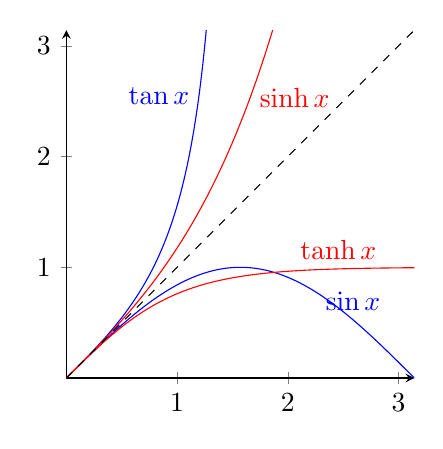
\begin{tikzpicture}
			\begin{axis}[
				axis lines=middle,
				ymin=0, ymax=pi,
				domain=0:pi,
				samples=100,
				width=6cm,
				height=6cm,
			]
			\addplot [blue, ] {sin(deg(x))} node [pos=.8,above] {$\sin x$};
			\addplot [blue, domain=0:1.5] {tan(deg(x))} node [pos=.2,left] {$\tan x$};
			\addplot [red, ] {sinh(x)} node [pos=.25,right] {$\sh x$};
			\addplot [red] {tanh(x)} node [pos=.8,above] {$\tanh x$};

			\addplot [black, dashed] {x};
			% \addplot [black, dashed, thick] {x + (x^3)/6} node [pos=.66,right] {$x + \dfrac{x^3}{3!}$};
			% \addplot [black, dashed, thick] {x - (x^3)/6} node [pos=.1,right] {$x - \dfrac{x^3}{3!}$};

			\end{axis}
		\end{tikzpicture}
	\end{aligned}
\] 

Tips to remember:
\begin{itemize}
	\item For $x^3$ level approximation, the \underline{inverse function} series are almost
		same except the \underline{sign of the cubic term reverses}.
	\item $\tan x$ and  $\sinh x$ are quicker to grow than $x$ so their cubic term is positive.
	\item $\tan$ like functions' cubic terms are no factorial denominators.
	
\end{itemize}

For hyperbolic functions, just change the sign of every second term(cubic term)
in the Taylor series of the corresponding trigonometric functions. Which comes from
the fact that
\[
	\sh x = -i \sin(ix), \quad \ch x = \cos(ix), \quad \th x = -i \tan(ix)
\] 
\subsection{Use the definition of integral to find limits}

A common type is
\[
	\lim_{n \to \infty} \frac{1}{n}\sum_{i=1}^n f\left(\frac{i}{n}\right)
	= \int_0^1 f(x) \dd x
\] 

But we should notice that we don't need the "variable" strictly in form of $\frac{i}{n}$, 
\begin{example}
	The limit
	\[
		I=\lim_{n \to \infty} \frac{1}{n}\sum_{i=1}^n
		\frac{i-\sin^2i}{n^2}\ln\left(1+\frac{i-\sin^2i}{n}\right)
	\] 
	can be rewrited as the integral
	\[
		I=\int _0^1 x \ln(1+x) \dd x
	\] 
	since we can let
	\[
		\xi_i=\frac{i-\sin^2i}{n}
	\] 
	then it is clear that
	\[
		\frac{i-1}{n} \leq \xi_i \leq \frac{i}{n}
	\] 
	which allows us(by Squeeze Theorem) to rewrite the sum as the integral.
	
\end{example}

\subsection{Useful Limits}

\begin{itemize}
	\item If $ a_1, a_2, \ldots, a_m > 0$, then
		\[
			\lim_{n \to \infty} \sqrt[n]{a_1^n + a_2^n + \ldots + a_m^n} = \max\{a_1, a_2, \ldots, a_m\}
		\]
		\begin{example}
			Find the limit
			\[
				\lim_{n \to \infty} \sqrt[n]{a^{-n} + b^{-n}}
			\]
			where $a>b>0$.
			\begin{answer}
				Since
				\[
					\sqrt[n]{a^{-n} + b^{-n}} = \sqrt[n]{\frac{1}{a^n} + \frac{1}{b^n}}
				\] 
				and $a^{-1} < b^{-1}$, we have
				\[
					\lim_{n \to \infty} \sqrt[n]{a^{-n} + b^{-n}} = b^{-1}
				\]
			\end{answer}
		\end{example}
		\begin{example}
			\[
				I=\lim_{n \to \infty} \sqrt[n]{1+|x|^{3n}}, \quad x \in \mathbb{R}
			\] 
			we have
			\[
				I = \begin{cases}
					1 & |x| \leq 1 \\
					|x|^3 & |x| > 1
				\end{cases}
			\]
		\end{example}
	\item If $ a_1, a_2, \ldots, a_m > 0$, then
		\[
			\lim_{n \to \infty} \left(\dfrac{a_1^{\frac{1}{n}} + a_2^{\frac{1}{n}} + \ldots + a_m^{\frac{1}{n}}}{m}\right)^n 
			=\sqrt[m]{a_1 a_2 \ldots a_m}
		\]
	\item when $n\to\infty$ we have Stirling's approximation:
		\[
			n! \sim \sqrt{2 \pi n} \left(\dfrac{n}{e}\right)^n
		\]
\end{itemize}

\subsection{Stolz Theorem}
If two sequences $\{x_n\}$ and $\{y_n\}$ satisfy:
\begin{itemize}
	\item $y_n$ and $x_n$ are both {strictly monotone increasing} and {unbounded},
		or both {strictly monotone decreasing} and tends to $0$;
	\item the limit $\lim_{n \to \infty} \dfrac{x_n - x_{n-1}}{y_n - y_{n-1}}$ exists or
		is equal to $\infty$ or $-\infty$;
\end{itemize}
then
\[
	\lim_{n \to \infty} \dfrac{x_n}{y_n} = \lim_{n \to \infty} \dfrac{x_n - x_{n-1}}{y_n - y_{n-1}}
\] 
especially, when $y_n = n$, we have
\[
	\lim_{n \to \infty} \dfrac{x_n}{n} = \lim_{n \to \infty} (x_n - x_{n-1})
\] 
\subsubsection{Dalembert-Cauchy}
\[
	\lim_{n \to \infty} \sqrt[n]{x_n} = \lim_{n \to \infty} \dfrac{x_n}{x_{n-1}}
\] 
since we can rewrite
\[
	\sqrt[n]{x_n} = \exp\left(\dfrac{\ln x_n}{n}\right) \to 
	\exp\left(\ln x_n - \ln x_{n-1}\right) = \dfrac{x_n}{x_{n-1}} = \dfrac{x_{n+1}}{x_n}
\]
In fact, this theorem is a indpendent result, not just a special case of Stolz Theorem.
But we do not claim it here.

\begin{example}
	Find the limit
	\[
		\lim_{n \to \infty} \frac{\sqrt[n]{n!}}{n}
	\] 
	\begin{answer}
		we have
		\[
			\lim_{n \to \infty} \sqrt[n]{\frac{n!}{n^{n}}}
		= \lim_{n \to \infty} \dfrac{(n+1)! / (n+1)^{n+1}}{n! / n^{n}}
		= \lim_{n \to \infty} \left(\dfrac{n}{n+1}\right)^{n}
		= e^{-1}
		\]
	\end{answer}
}
	
\end{example}

\section{Function}

\subsection{Identity equation}

Inverse trigonometric functions satisfy the following identities:
\begin{itemize}
	\item $\arctan \dfrac{1}{x}$ is not always equal to $\arccot x$, actually
		\[
			\arctan \dfrac{1}{x} = \begin{cases}
			\dfrac{\pi}{2} - \arctan x & x > 0 \\
			\\
			-\dfrac{\pi}{2} - \arctan x & x < 0
		\end{cases} \quad
			\begin{aligned}
		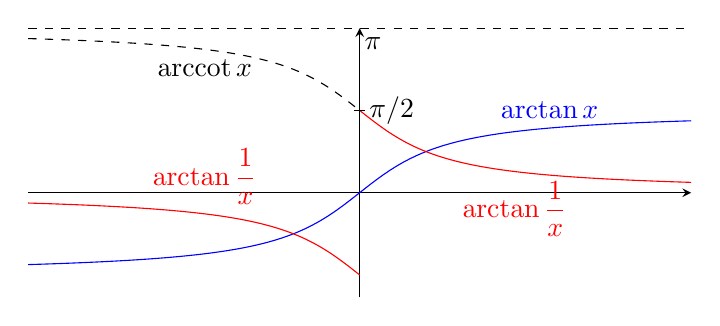
\begin{tikzpicture}
			\begin{axis}[
				axis lines=middle,
				xtick=\empty,ytick=\empty,
				ymin=-2, ymax=pi,
				domain=-5:5,
				samples=100,
				width=10cm,
				height=5cm,
			]
			\addplot [blue, ] {rad(atan(x))} node [pos=.8,above] {$\arctan x$};
			\addplot [red, domain=-5:0] {rad(atan(1/x))} node [pos=.5, above] {$\arctan \dfrac{1}{x}$};
			\addplot [red, domain=0:5] {rad(atan(1/x))} node [pos=.5, below] {$\arctan \dfrac{1}{x}$};
			\addplot [dashed, domain=-5:0] {pi/2-rad(atan(x))} node [pos=.5, below] {$\arccot x$};
			\addplot [dashed] {pi} node [pos=.52,below] {$\pi$};
			
			\addplot [only marks, mark=-] coordinates {(0,pi/ 2)} node[right] {$\pi/2$};

			\end{axis}
		\end{tikzpicture}
			\end{aligned}
		\] 
		since $\arctan x$ only takes values in $\left(-\dfrac{\pi}{2}, \dfrac{\pi}{2}\right)$,
		while $\arccot x$ takes values in $(0, \pi)$.
	\item $\arcsin x + \arccos x = \dfrac{\pi}{2}$
	\item $\arctan x + \arccot x = \dfrac{\pi}{2}$
	\item $\arctan\dfrac{a+b}{1-ab} = \arctan a + \arctan b$, \underline{\textbf{when $ab<1$}}.
		\[
		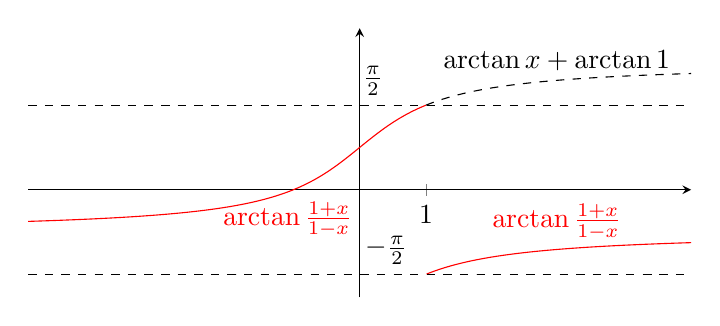
\begin{tikzpicture}
			\begin{axis}[
				axis lines=middle,
				xtick={1},ytick=\empty,
				ymin=-2, ymax=3,
				domain=-5:5,
				samples=100,
				width=10cm,
				height=5cm,
			]
			\addplot [dashed, domain=1:5] {rad(atan(x))+pi / 4} node [pos=.5,above] {$\arctan x + \arctan 1$};
			\addplot [red, domain=-5:1] {rad(atan((1+x)/(1-x)))} node [pos=.6, below] {$\arctan \frac{1+x}{1-x}$};
			\addplot [red, domain=1.01:5] {rad(atan((1+x)/(1-x))} node [pos=.5, above] {$\arctan \frac{1+x}{1-x}$};
			\addplot [dashed] {pi / 2} node [pos=.52,above] {$\frac{\pi}{2}$};
			\addplot [dashed] {-pi / 2} node [pos=.54,above] {$-\frac{\pi}{2}$};
			
			% \addplot [only marks, mark=-] coordinates {(0,pi/ 2)} node[right] {$\pi/2$};

			\end{axis}
		\end{tikzpicture}
		\] 
\end{itemize}

When dealing with sine function, we have
\begin{itemize}
	\item $\sin x= (-1)^{n}\sin(x-n\pi)$, for any integer $n$. It is very useful
		to deal with n in sine function, not only in limits but also in series.
		\begin{example}
			Find the limit
			\[
				\lim_{n \to \infty} \sin^2\left(\pi \sqrt{n^2 + n}\right)
			\]
			we have
			\[
				\sin^2\left(\pi \sqrt{n^2 + n}\right)
				=\sin^2\left(\pi \left(\sqrt{n^2 + n} - n\right)\right)
			\]
			since
			\[
				\sqrt{n^2 + n} - \sqrt{n^2} = \dfrac{1}{2\sqrt{\xi}}n \to \frac{1}{2}
			\]
			for some $\xi \in (n^2, n^2+n)$ by Mean Value Theorem, we have
			\[
				\lim_{n \to \infty} \sin^2\left(\pi \sqrt{n^2 + n}\right)
				= \sin^2\left(\frac{\pi}{2}\right) = 1
			\]
		\end{example}
	\item $\tan x = \tan(x-n\pi)$, for any integer $n$.
		\begin{example}
			Find the limit
			\[
				\lim_{n \to \infty} n \tan\left(\pi \sqrt{n^2 + 1}\right)
			\]
			we have
			\[
				n \tan\left(\pi \sqrt{n^2 + 1}\right)
				=n \tan\left(\pi \left(\sqrt{n^2 + 1} - n\right)\right)
			\]
			since
			\[
				\sqrt{n^2 + 1} - \sqrt{n^2} = \dfrac{1}{2\sqrt{\xi}} \to \frac{1}{2n}
			\]
			for some $\xi \in (n^2, n^2+1)$. So
			\[
				\lim_{n \to \infty} n \tan\left(\pi \sqrt{n^2 + 1}\right)
				= \lim_{n \to \infty} n \tan\left(\frac{\pi}{2n}\right)
				= \frac{\pi}{2}
			\]
		\end{example}
	
\end{itemize}

\subsection{Inequalities}

\begin{itemize}
	\item For $0<x<\dfrac{\pi}{2}$, we have
		\[
			\sin x < x < \tan x
		\]
		and
		\[
			\begin{array}{c}
				\dfrac{2}{\pi} x < \sin x < x \\
				\sin x < x < \dfrac{\pi}{2} \sin x
			\end{array}\quad
			\begin{aligned}
				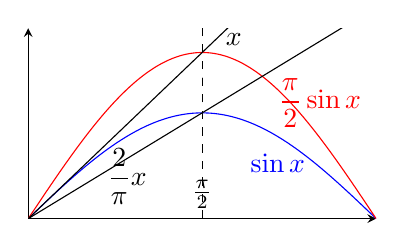
\begin{tikzpicture}
					\begin{axis}[
						axis lines=middle,
						xtick=\empty,ytick=\empty,
						ymin=0, ymax=1.8,
						domain=0:pi,
						samples=100,
						width=6cm,
						height=4cm,
					]
					\addplot [domain=0:2*pi,dashed] ({pi / 2}, {x}) node [pos=0,above] {$\frac{\pi}{2}$};
					\addplot [blue, ] {sin(deg(x))} node [pos=.8,left] {$\sin x$};
					\addplot [red] {pi/ 2 *sin(deg(x))} node [pos=.8,above] {$\dfrac{\pi}{2}\sin x$};
					\addplot [black, ] {2 / pi *x} node [pos=.2,right] {$\dfrac{2}{\pi} x$};
					\addplot [black] {x} node [pos=.54,right] {$x$};
					\end{axis}
				\end{tikzpicture}
			\end{aligned}
		\] 
		\begin{example}
			Given $\{x_n\},\{y_n\}$ satisfy $x_1=y_1=\frac{1}{2}$, and $x_{n+1}=\sin x_n, 
			y_{n+1}=y_n^2 $ try to compare their order of infinitesimal.
			\begin{answer}
				Since $0<x_n<\frac{\pi}{2}$ we have
				\[
					x_{n+1}=\sin x_n > \dfrac{2}{\pi} x_n > \cdots > \left(\dfrac{2}{\pi}\right)^{n-1} x_1
				\] 
				while $0<y_n\leq \frac{1}{2}$ so
				\[
					y_{n+1} = y_n\cdot y_n \leq \dfrac{1}{2} y_n \leq \cdots \leq \left(\dfrac{1}{2}\right)^{n-1} y_1
				\]
				thus
				\[
					0\leq\lim_{n \to \infty} \dfrac{y_n}{x_n} \leq \lim_{n \to \infty} \dfrac{\left(\frac{1}{2}\right)^{n-1} y_1}
					{\left(\frac{2}{\pi}\right)^{n-1} x_1} = 0
				\]
				that is, $y_n$ is a higher order infinitesimal than $x_n$.
			\end{answer}
			
		\end{example}
	\item For $x>-1$, we have
		\[
			\dfrac{x}{1+x} < \ln(1+x) < x \quad
			\begin{aligned}
				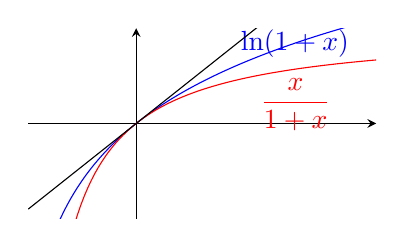
\begin{tikzpicture}
					\begin{axis}[
						axis lines=middle,
						xtick=\empty,ytick=\empty,
						ymin=-1, ymax=1,
						domain=-0.9:2,
						samples=100,
						width=6cm,
						height=4cm,
					]
					\addplot [blue, ] {ln(x + 1)} node [pos=.85] {$\ln(1+x)$};
					\addplot [red] {x / (x + 1)} node [pos=.94,below] {$\dfrac{x}{1+x}$};
					\addplot [black] {x};
					\end{axis}
				\end{tikzpicture}
			\end{aligned}
		\] 
\end{itemize}

for ceiling function and floor function, we have
\[x-1 < \lfloor x \rfloor \leq x \leq \lceil x \rceil < x+1\]
\begin{example}
	Find the limit
	\[
		\lim_{x \to 0} x \left\lfloor \dfrac{2}{x} \right\rfloor
	\] 
	\begin{answer}
		Since
		\[
			\dfrac{2}{x} - 1 < \left\lfloor \dfrac{2}{x} \right\rfloor \leq \dfrac{2}{x}
		\] 
		when $x>0$, we have
		 \[
			2 - x < x \left\lfloor \dfrac{2}{x} \right\rfloor \leq 2
		\] 
		telling us that
		\[
			\lim_{x \to 0^+} x \left\lfloor \dfrac{2}{x} \right\rfloor = 2
		\]
		when $x<0$, in a similar way we can get the limit is $2$
	\end{answer}
\end{example}

\subsection{Periodic Function}
A antiderivative of a periodic function is a periodic function plus a linear function.
The antiderivative of periodic function is periodic if and only if the integral over
one period is zero.

And here are some sufficient conditions to make the integral over one period zero:
\begin{itemize}
	\item If $f(x)$ is an odd function, since
		\[
			\int_0^T f(x)\dd x=\int_{-T/2}^{T/2} f(x)\dd x=0
		\] 
	\item If the improper integral
		\[
			\int_0^\infty f(x)\dd x
		\] 
		converges. Since it can be written as
		\[
			\int_0^\infty f(x)\dd x = \lim_{n \to \infty} \int_0^{nT} f(x)\dd x = \lim_{n \to \infty} n \int_0^T f(x)\dd x
		\] 
		if $\int_0^T f(x)\dd x \neq 0$, the improper integral will diverge.

\end{itemize}

\subsection{Bounded and Unbounded Function}
\subsubsection{Bounded Function}

\begin{itemize}
	\item If $f(x)$ is continous on  $[a, b]$, then $f(x)$ is bounded on $[a, b]$.
	\item If $f(x)$ is continous on $(a, b)$, and $\lim_{x \to a^+} f(x)$ and
		$\lim_{x \to b^-} f(x)$ exist and are finite, then $f(x)$ is bounded on $(a, b)$.
		Note that this is not iff condition, when the limits do not exist but bounded,
		$f(x)$ may still be bounded on $(a, b)$.
	\item If $f'(x)$ is bounded on finite interval $I$, then $f(x)$ is bounded on $I$.
		This can be shown using Mean Value Theorem. And this property can be useful
		when $f(x)$ is defined as an integral.
		\begin{example}
			Consider the function
			\[
				f(x) = \int_0^x \frac{\sin(x)}{x} \dd x \quad x \in (0, 2024)
			\]
			Since
			\[
				f'(x) = \frac{\sin(x)}{x}
			\]
			is bounded on $(0, 2024)$, $f(x)$ is also bounded on $(0, 2024)$.

			
		\end{example}

\end{itemize}

A function is bounded can not guarantee that the limit exists, an classic example
is the function $\sin x$.

\subsubsection{Unbounded Function}

An unbounded function only requires that for any large number $M>0$, there exists
some $x$ such that $|f(x)|>M$. It does not require that as $x \to \infty$, $|f(x)| \to \infty$.
In a other word, an unbounded function only requires existence of some subsequence
make the function value grow without bound, limits along other subsequences can be finite.
But if we require that as $x \to \infty$, $|f(x)| \to \infty$, every subsequence must
also diverge to infinity.

\begin{example}
	Consider the function
	\[
		f(x) = x \sin x
	\] 
	This function is unbounded since we can choose $x_n = 2n\pi + \dfrac{\pi}{2}$,
	then
	\[
		|f(x_n)| = \left| \left(2n\pi + \dfrac{\pi}{2}\right) \sin\left(2n\pi + \dfrac{\pi}{2}\right) \right| = 2n\pi + \dfrac{\pi}{2} \to \infty
	\]
	as $n \to \infty$. However, if we choose another subsequence $x_n = 2n\pi$,
	then
	\[
		|f(x_n)| = \left| \left(2n\pi\right) \sin\left(2n\pi\right) \right| = 0
	\]
	for all $n$. And so this function is unbounded, but does not diverge to infinity as $x \to \infty$.
\end{example}

\subsection{Variable limit integral}

\begin{lemma}\label{lem:varLimIntDeriv}
Taking the derivative with a variable independent of the integration variable can be moved into the integral:
\[
	\dfrac{\dd}{\dd y} \int_a^b f(x, y) \dd x = \int_a^b f_y(x, y) \dd x
\] 
here we don't give the proof.
\end{lemma}
\begin{theorem}[Leibniz Integral Rule]
If $f(x, t)$ and $f_x(x, t)$
are continuous on $[a(x), b(x)]$, then
\[
	\frac{\dd}{\dd x} \int_{a(x)}^{b(x)} f(x, t) \dd t
	= \int_{a(x)}^{b(x)} f_x(x, t) \dd t
	+ f(x, b(x)) b'(x) - f(x, a(x)) a'(x)
\]
where $f_x(x, t) = \partial f(x, t)/\partial x$.
\begin{proof}
	Let $F(x, t)$ denote the antiderivative of $f(x, t)$ with respect to $t$:
	\[
		F(x, t) = \int_{0}^{t} f(x, s) \dd s + C(x) = \int f(x, t) \dd t
	\] 
	then we can write the integral with variable limits as
	\[
		I = \int_{a(x)}^{b(x)} f(x, t) \dd t = F(x, b(x)) - F(x, a(x))
	\]
	then taking derivative with respect to $x$ and $t$, we have (using Lemma \ref{lem:varLimIntDeriv}):
	\[
		F_x = \int f_x(x, t) \dd t \quad \text{and} \quad F_t = f(x, t)
	\] 
	then using the chain rule of multivariable function, we have
	\[
		\begin{aligned}
			\dfrac{\dd I}{\dd x} &= \dfrac{\dd}{\dd x} F(x, b(x)) - \dfrac{\dd}{\dd x} F(x, a(x)) \\
			&= F_x(x, b(x)) + F_t(x, b(x)) b'(x)
			- F_x(x, a(x)) - F_t(x, a(x)) a'(x) \\
			&= \int_{a(x)}^{b(x)} f_x(x, t) \dd t
			+ f(x, b(x)) b'(x) - f(x, a(x)) a'(x)
		\end{aligned}
	\]
\end{proof}
\end{theorem}
Especially, when $a(x)=0$ and $b(x)=x$, we have
\begin{theorem}
	\[
		\frac{\dd}{\dd x} \int_{0}^{x} f(x, t) \dd t
		= \int_{0}^{x} f_x(x, t) \dd t
		+ f(x, x)
	\]
\end{theorem}

But when $f(x, t)$ is not explicitly defined, for example, defined with abstract function,
we had better use variable substitution to convert it has no integration variable in the abstract function.
and use normal Leibniz Integral Rule, since abstract function's derivative gives no useful information.

\subsection{Mean Value Theorem for Integrals}
If $f(x)$ is continuous on $[a, b]$, then there exists some $\xi \in [a, b]$ such that
\[
	\int_a^b f(x) \dd x = f(\xi)(b-a)
\]
Be careful on limit case,we can not say $\xi\sim$ $a$ or $\xi\sim b$ or other expressions
even if $a$ or $b$ tends to same limit, that is, when $a \to A$ and $b \to A$, 
we only have $\xi \to A$, but we can not determine how $\xi$ approaches $A$.
\begin{example}
	Find the limit when $f (x)\sim x$ near $0$
	\[
		\lim_{x \to 0} \frac{\int_0^x e^{-t} f(t) \dd t}{t^2}
	\]
	Using Mean Value Theorem for Integrals, there exists some $\xi \in [0, x]$ such that
	\[
		\int_0^x e^{-t} f(t) \dd t = e^{-\xi} f(\xi) x
	\]
	but we can not say $\xi \sim x$ and substitute $x$ into $f$ directly, which gives
	the wrong answer. Since as $x \to 0$, we only have $\xi \to 0$, so this
	only gives an undeterminate form and we need to use another method to solve it.
\end{example}

Another Mean Value Theorem for Integrals is:
\begin{theorem}
	If $f(x)$ is continuous and bounded on $[a, b]$, and $g(x)$ is integrable
	and does not change sign on $[a, b]$, then there exists some $\xi \in [a, b]$
	such that
	\[
		\int_a^b f(x) g(x) \dd x = f(\xi) \int_a^b g(x) \dd x
	\]
	which can be proved using the Intermediate Value Theorem.
\end{theorem}
\begin{example}
	Find the limit
	\[
		\lim_{x \to 0} \int_0^1 x^{n} \sqrt{1+x^2} \dd x
	\]
	Since $\sqrt{1+x^2}$ is continuous and bounded on $[0, 1]$, and
	$x^{n}$ does not change sign, there exists some $\xi \in [0, 1]$ such that
	\[
		\int_0^1 x^{n} \sqrt{1+x^2} \dd x = \sqrt{1+\xi^2} \int_0^1 x^{n} \dd x
		= \sqrt{1+\xi^2} \cdot \frac{1}{n+1}
	\]
	as $n \to \infty$, we have $\sqrt{1+\xi^2} \to \sqrt{2}$ is bounded, so
	\[
		\lim_{x \to 0} \int_0^1 x^{n} \sqrt{1+x^2} \dd x = 0
	\]
\end{example}

\begin{example}
	Find the limit
	\[
		I=\lim_{n \to \infty} \int_1^{\sqrt3} \dfrac{\sqrt[n]{x}}{1+x^2} \dd x
	\]
	Since $\sqrt[n]{x}$ is continuous and bounded on $[1, \sqrt3]$, and
	$\dfrac{1}{1+x^2}$ does not
	change sign, there exists some $\xi \in [1, \sqrt3]$ such that
	\[
		\int_1^{\sqrt3} \dfrac{\sqrt[n]{x}}{1+x^2} \dd x
		= \sqrt[n]{\xi} \int_1^{\sqrt3} \dfrac{1}{1+x^2} \dd x
		= \frac{\pi}{12}\sqrt[n]{\xi}
	\]
	as $n \to \infty$, we have $\sqrt[n]{\xi} \to 1$, so the limit is $\dfrac{\pi}{12}$.
\end{example}
	

\end{document}
